%========================================
\chapter{RESULTS}
\label{ch:resu}
%========================================

Results are presented in this chapter for the previous work, application of a PINN implementation for the 1D Burgers equation, and the current preliminary work, the DNN-based gas optics implementation.


%========================================
\section{PINN Implementation for the 1D Burgers Equation}
%========================================

The results for the 1D Burger's equation are divided into two parts of experiments: 
(i) the first compares the results of PINN with the 4 SINDy versions; 
(ii) the second evaluates the PINN implementation for various hyperparameters and CP sizes.

The first part uses datasets related to different problem sizes ($x$ space versus $t$ time discretization): 128x64, 256x128, and 512x256, while the second part uses only a 256x100 problem size. The GQM is used to generate the dataset corresponding to the exact solution (reference), which are then employed by the SINDy versions, and also to extract the set of CPs used by the PINN implementation. The MLP architecture used for the PINN implementation in the first part has one input layer, 3 hidden layers with 20 neurons each, and one output layer. The PINN undergoes training and PDE parameters are estimated, solving the inverse problem, and the resulting model estimates the solution (space versus time field). The processing-time data obtained in the all experiments is given by the average of 3 executions. 

%========================================
\subsection{Comparison of PINN and SINDy parameter discovery}
%========================================

Tables \ref{tab:nm-pinn-time-comp-01} and \ref{tab:nm-pinn-time-comp-02} show  the average of elapsed times of 3 runs on the local machine for the PINN (using GPU) and the 4 SINDy implementations (only CPU), for the 3 problem sizes and for the two cases of viscosity.  In the case of PINN, training time to estimate the parameters and prediction time of the resulting 1D field using the trained model are shown. Processing times of SINDy versions are consistently lower than those of the PINN model, even considering that the latter executes using GPU. Therefore, future studies must consider the tradeoff between accuracy and processing times when comparing PINNs and numerical methods like SINDy. 

\begin{table}[htb]\centering
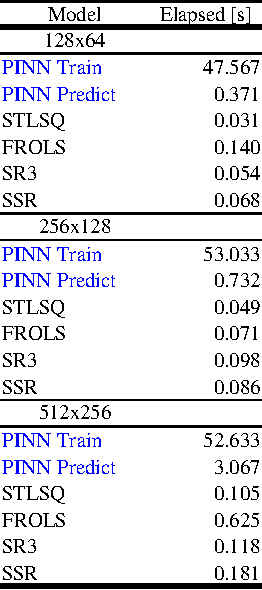
\includegraphics[width=.27\columnwidth]{nm-pinn-time-comp-01}
\vspace{1em}
\caption{Comparison of elapsed times (average of 3 runs) for the PINN and the 4 SINDy models for kinematic viscosity of the fluid of ${0.01}/{\pi}$, and for execution on the local machine (PC).}
\label{tab:nm-pinn-time-comp-01}
\end{table}

\begin{table}[htb]\centering
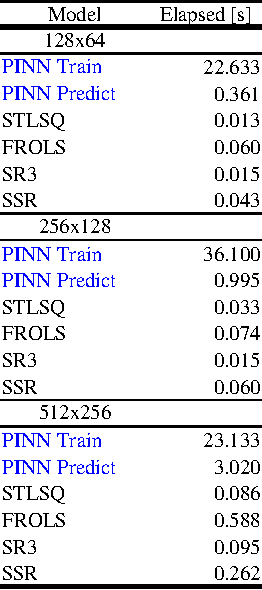
\includegraphics[width=.27\columnwidth]{nm-pinn-time-comp-02}
\vspace{1em}
\caption{Comparison of elapsed times (average of 3 runs) for the PINN and the 4 SINDy models for kinematic viscosity of the fluid of ${0.1}/{\pi}$, and for execution on the local machine (PC).}
\label{tab:nm-pinn-time-comp-02}
\end{table}

Tables \ref{tab:nm-pinn-01} and \ref{tab:nm-pinn-02} show the results obtained for the PDE parameter discovery, comparing the  PINN and the 4 SINDy implementations (STLSQ, FROLS, SR3 and SSR, discussed in \autoref{sec:npd}), and also considering 2 different viscosity values in the 1D Burgers' equation, ${0.01}/{\pi}$ and ${0.1}/{\pi}$. As already commented, 3 sizes of problems are considered: 128x64, 256x128 and 512x256. 

Subscripts denote partial differentiation in time and space, e.g. u\_x denotes ${du}/{dx}$, u\_xx denotes ${d^2u}/{dx^2}$, and so on. -At the top of each table is shown the \textit{Exact PDE} 1D Burgers' equation (e.g., $u_t + 1.0 u u_x - 0.003183 u_{xx} = 0$) used to generate the datasets.

In the case of PINN, training is done using 2,000 CPs randomly obtained from the dataset, regardless of the size of the problem.  In the case of SINDy implementations, the complete dataset is used in the model to obtain the parameters. In \ref{tab:nm-pinn-01} the viscosity value (${0.01}/{\pi}$) is lower than in the second (${0.1}/{\pi}$) in order to check if SINDy accuracy is compromised for  small viscosity values, as confirmed by the results. PINN accuracy was good, even using the set of CPs extracted from the smaller dataset, and such accuracy improves with the problem size. \ref{tab:nm-pinn-01} is for experiments with the higher viscosity value, showing that the accuracy of the SINDy implementations improved in comparison to the results of the preceding table, but are still lower than those obtained by PINN.

\begin{table}[htb]\centering
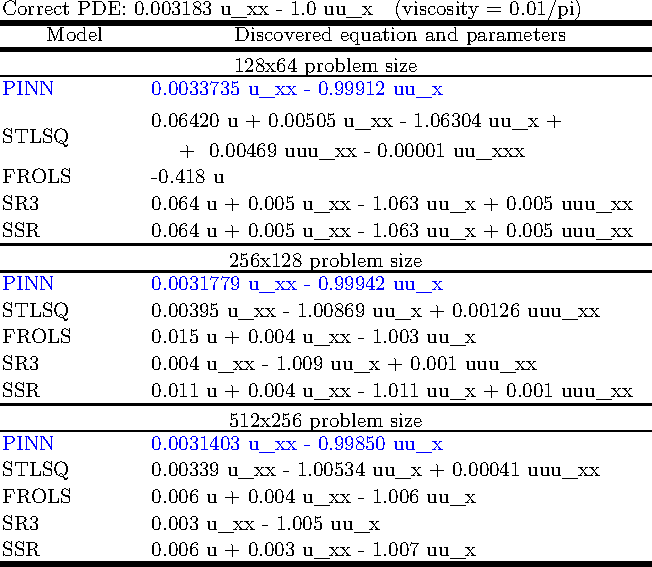
\includegraphics[width=.7\columnwidth]{nm-pinn-01}
\vspace{1em}
\caption{Comparison of the results of the parameter discovery for the 1D Burgers' equation using PINN (in blue) and the 4 SINDy versions (kinematic viscosity of the fluid of ${0.01}/{\pi}$).}
\label{tab:nm-pinn-01}
\end{table}

\begin{table}[htb]\centering
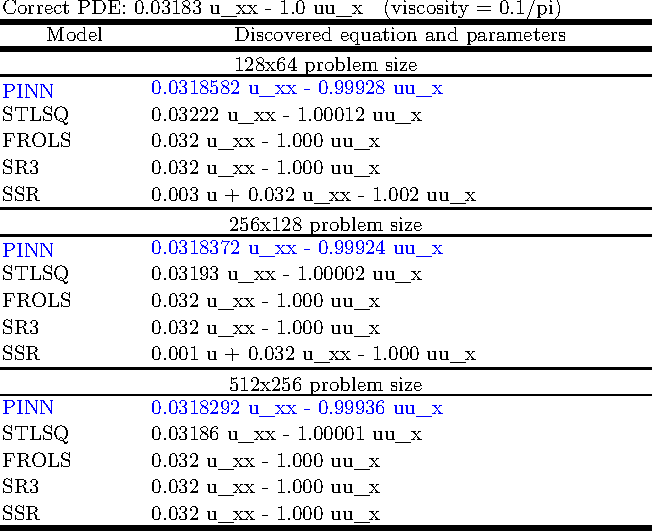
\includegraphics[width=.7\columnwidth]{nm-pinn-02}
\vspace{1em}
\caption{Comparison of the results of the parameter discovery for the 1D Burgers' equation using PINN (in blue) and the 4 SINDy versions (kinematic viscosity of the fluid of ${0.1}/{\pi}$).}
\label{tab:nm-pinn-02}
\end{table}

The next subsections present the solution field $u(t,x)$ generated by the PINN implementation for the 3 problem sizes, and for the 2 viscosity values. For each case, there are figures showing the predicted solution $u(t,x)$ with marks representing the CPs, and a particular snapshot at time $t=0.5$ comparing the PINN prediction and the exact solution. These figures allow a visual assessment of the accuracy of the solutions.

\FloatBarrier

%========================================
\subsubsection{Problem Size 128x64}
%========================================

Figures \ref{fig:pinn-01-128-a}, \ref{fig:pinn-01-128-b}, \ref{fig:pinn-02-128-a}, and \ref{fig:pinn-02-128-b} show, for the problem size 128x64, the solutions for the viscosities ${0.01}/{\pi}$ and ${0.1}/{\pi}$. Figures \ref{fig:pinn-01-128-a} and \ref{fig:pinn-02-128-a} show the predicted spatio-temporal solution $u(t, x)$, and the CPs used to training are represented as dark marks on the graph. Since the dataset is relatively small and the number of CP is 2,000, the small marks are aligned and may not appear random at first. 
At the top and bottom of the figure, ($x=1.0$ and $x=-1.0$), are the CPs related to the boundary conditions (BC) of the PDE, on the left side ($t=0, 0$) are the CPs relative to the initial conditions (IC), and in the center of the figure ($x=0.0$) the complex non-linear behavior (sometimes called formation of a shock wave) of the Burgers' equation with lower viscosity is represented. The remaining randomly selected CPs appear on the graph. Although it was not done this way, it is possible to select more points in the BC and IC regions to reinforce network training, if necessary.

Figures \ref{fig:pinn-01-128-b} and \ref{fig:pinn-02-128-b} show a snapshot in time comparing the superimposed solution for the PINN method and the exact numerical solution.
It is possible to see that even using a few CPs, the PINN was able to accurately capture the complex non-linear behavior of the Burgers' equation, which presents the formation of an accentuated internal layer around t = 0.4, which is generally difficult to solve with traditional NM and requires a laborious spatio-temporal discretization of the equation. 
In this scenario, we can directly address the nonlinear problem without needing to commit to any prior assumptions, linearization, or local time step.

\begin{figure}[htb]\begin{minipage}[b]{\textwidth}\centering
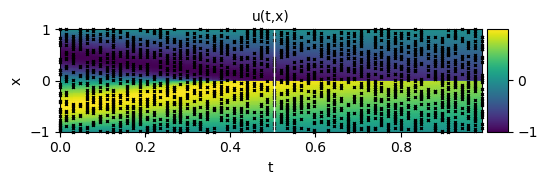
\includegraphics[width=.75\columnwidth]{pinn-01-128-a}
\vspace{-1em}
\caption{PINN predicted solution $u(t, x)$ for viscosity ${0.01}/{\pi}$ and problem size 128x64.}
\label{fig:pinn-01-128-a}
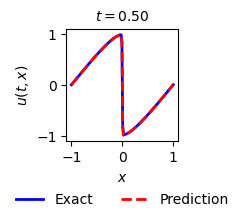
\includegraphics[width=.4\columnwidth]{pinn-01-128-b}
\vspace{-1em}
\caption{Comparison of the solutions obtained by PINN (in red) and the exact numerical solution (in blue) for the $t=0.5$ snapshot (viscosity of ${0.01}/{\pi}$ and problem size of 128x64).}
\label{fig:pinn-01-128-b}
\end{minipage}\end{figure}

\begin{figure}[htb]\begin{minipage}[b]{\textwidth}\centering
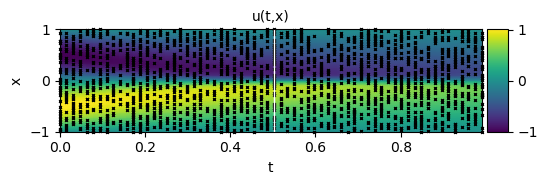
\includegraphics[width=.75\columnwidth]{pinn-02-128-a}
\vspace{-1em}
\caption{PINN predicted solution $u(t, x)$ for viscosity ${0.1}/{\pi}$ and problem size 128x64.}
\label{fig:pinn-02-128-a}
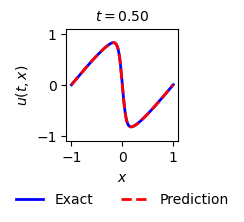
\includegraphics[width=.4\columnwidth]{pinn-02-128-b}
\vspace{-1em}
\caption{Comparison of the solutions obtained by PINN (in red) and the exact numerical solution (in blue) for the $t=0.5$ snapshot (viscosity of ${0.1}/{\pi}$ and problem size of 128x64).}
\label{fig:pinn-02-128-b}
\end{minipage}\end{figure}

Due to the number of CPs being constant even when the size of the dataset varies, great variation in the discovery of parameters in the PINN model is not expected. In the case of the NMs seen in Tables \ref{tab:nm-pinn-01} and \ref {tab:nm-pinn-02}, the variation is expected because the NM uses the complete dataset (does not use CP). In addition, there is also variation related to each NM algorithm. For the \autoref{tab:nm-pinn-01} with lower viscosity, it is possible to observe that for 128x64 (total of 8,192 data points) the accuracy of the NM was not good, unlike the PINN model which obtained good accuracy even with a smaller amount (2000 CPs) of training data. As for \autoref{tab:nm-pinn-02} with higher viscosity, it is possible to observe that for 128x64 the NM showed better accuracy, especially FROLS and SR3, approaching the PINN model.

\FloatBarrier

%========================================
\subsubsection{Problem Size 256x128}
%========================================

The Figures \ref{fig:pinn-01-256-a}, \ref{fig:pinn-01-256-b}, \ref{fig:pinn-02-256-a} and \ref{fig:pinn-02-256-b} show, for the problem size 256x128, the solutions for the viscosities ${0.01}/{\pi}$ and ${0.1}/{\pi}$. Much of what was presented in the previous section also applies to this section. In Figures \ref{fig:pinn-01-256-a} and \ref{fig:pinn-02-256-a} one can initially observe a better distribution of CPs in a more random way, due to the fact that the set of data to be larger and the size of the CP set remains at 2,000 CPs, allowing the CP to be distributed a little better in the graph. Figures \ref{fig:pinn-01-256-b} and \ref{fig:pinn-02-256-b} show the same behavior as the previous subsection, even because the amount of CP is the same. For the \autoref{tab:nm-pinn-01} with lower viscosity, and 256x128 problem size, the NMs were not accurate. For low viscosity, in most cases, regardless of the dataset, the PINN model showed better accuracy. For the \autoref{tab:nm-pinn-02} with higher viscosity, and 256x64 problem size, most of the NMs behaved well, differently from what occurs in the case with lower viscosity.

\begin{figure}[htb]\begin{minipage}[b]{\textwidth}\centering
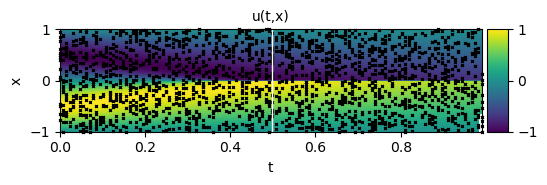
\includegraphics[width=.75\columnwidth]{pinn-01-256-a}
\vspace{-1em}
\caption{PINN predicted solution $u(t, x)$ for viscosity ${0.01}/{\pi}$ and problem size 256x128.}
\label{fig:pinn-01-256-a}
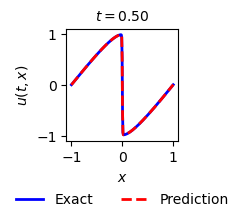
\includegraphics[width=.4\columnwidth]{pinn-01-256-b}
\vspace{-1em}
\caption{Comparison of the solutions obtained by PINN (in red) and the exact numerical solution (in blue) for the $t=0.5$ snapshot (viscosity of ${0.01}/{\pi}$ and problem size of 256x128).}
\label{fig:pinn-01-256-b}
\end{minipage}\end{figure}

\begin{figure}[htb]\begin{minipage}[b]{\textwidth}\centering
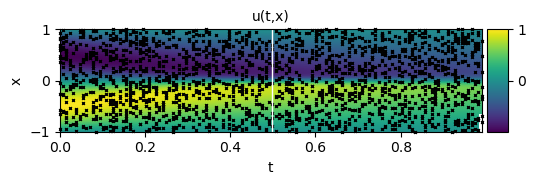
\includegraphics[width=.75\columnwidth]{pinn-02-256-a}
\vspace{-1em}
\caption{PINN predicted solution $u(t, x)$ for viscosity ${0.1}/{\pi}$ and problem size 256x128.}
\label{fig:pinn-02-256-a}
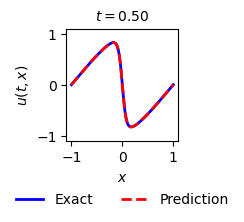
\includegraphics[width=.4\columnwidth]{pinn-02-256-b}
\vspace{-1em}
\caption{Comparison of the solutions obtained by PINN (in red) and the exact numerical solution (in blue) for the $t=0.5$ snapshot (viscosity of ${0.1}/{\pi}$ and problem size of 256x128).}
\label{fig:pinn-02-256-b}
\end{minipage}\end{figure}

%========================================
\subsubsection{Problem Size 512x256}
%========================================

The Figures \ref{fig:pinn-01-512-a}, \ref{fig:pinn-01-512-b}, \ref{fig:pinn-02-512-a} and \ref{fig:pinn-02-512-b} show, for the problem size 512x256, the same behavior as the previous subsection. For Tables \ref{tab:nm-pinn-01} and \ref{tab:nm-pinn-02}, 512x256 problem size, the NMs showed similar behavior to the previous section, with the SSR method standing out.

\begin{figure}[htb]\begin{minipage}[b]{\textwidth}\centering
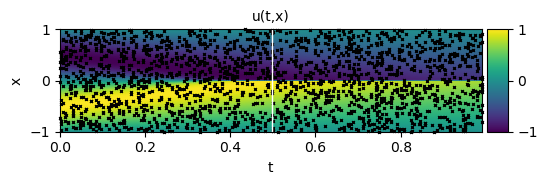
\includegraphics[width=.75\columnwidth]{pinn-01-512-a}
\vspace{-1em}
\caption{PINN predicted solution $u(t, x)$ for viscosity ${0.01}/{\pi}$ and problem size 512x256.}
\label{fig:pinn-01-512-a}
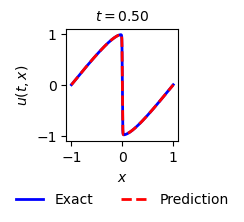
\includegraphics[width=.4\columnwidth]{pinn-01-512-b}
\vspace{-1em}
\caption{Comparison of the solutions obtained by PINN (in red) and the exact numerical solution (in blue) for the $t=0.5$ snapshot (viscosity of ${0.01}/{\pi}$ and problem size of 512x256).}
\label{fig:pinn-01-512-b}
\end{minipage}\end{figure}

\begin{figure}[htb]\begin{minipage}[b]{\textwidth}\centering
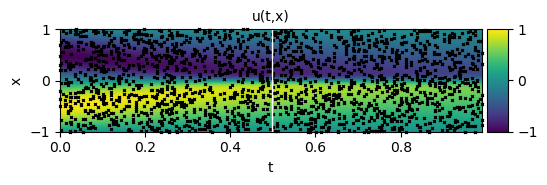
\includegraphics[width=.75\columnwidth]{pinn-02-512-a}
\vspace{-1em}
\caption{PINN predicted solution $u(t, x)$ for viscosity ${0.1}/{\pi}$ and problem size 512x256.}
\label{fig:pinn-02-512-a}
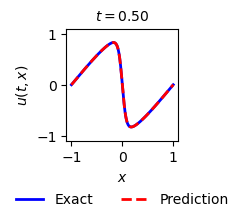
\includegraphics[width=.4\columnwidth]{pinn-02-512-b}
\vspace{-1em}
\caption{Comparison of the solutions obtained by PINN (in red) and the exact numerical solution (in blue) for the $t=0.5$ snapshot (viscosity of ${0.1}/{\pi}$ and problem size of 512x256).}
\label{fig:pinn-02-512-b}
\end{minipage}\end{figure}

\FloatBarrier

%========================================
\subsection{Evaluation of PINN Hyperparameters and CP Size}
%========================================

PINN processing time and accuracy is evaluated using the model generated with different sets of hyperparameters and CP set sizes in experiments executed on SDumont. Resulting predicted 1D fields are presented in figures, which are similar to those of the previous section. Following, PINN accuracy and processing times are evaluated as a function of the number of neurons per hidden layer, the number of hidden layers, and also the size of the CP set.

%========================================
\subsubsection{Visual Assessment of PINN}
%========================================

In this section, the network architecture is the same employed for the preceding comparisons between PINN and SINDy implementations (single input and output layers and 4 hidden layers with 20 neurons each). A visual assessment of predictive accuracy for problem size 256x100 and fluid viscosity of 0.01 is shown in \autoref{fig:bur1}, with time $t$ on the horizontal axis and spatial coordinate $x$ on the vertical axis. The color scale refers to the velocity $u(t, x)$. The black dots on the graph represent the 2,000 CPs randomly generated from the dataset and used for training. The \autoref {fig:bur2} shows a specific snapshot at $t=0.5$, where it is possible to observe the overlapping solutions for PINN and GQM (exact).  For this specific result, the equation obtained by PINN is $u_t + 0.99967 u u_x - 0.0030988 u_{xx} = 0$, while the exact PDE is $u_t + u u_x - 0 ,0031831 u_{xx} = 0$. Thus, the PINN could identify the underlying PDE with good accuracy.

\begin{figure}[htb]\begin{minipage}[b]{\textwidth}\centering
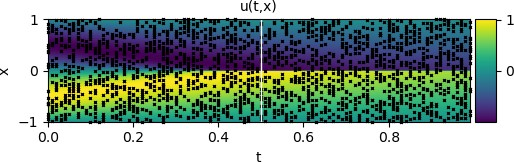
\includegraphics[width=.75\columnwidth]{burg-01.jpg}
\vspace{0em}
\caption{PINN predicted solution $u(t, x)$ for viscosity ${0.01}/{\pi}$ and problem size 256x100 (black dots denote the 2,000 randomly assigned CPs).} 
\label{fig:bur1}
\vspace{1em}
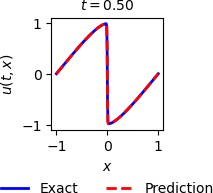
\includegraphics[width=.35\columnwidth]{burg-02.jpg}
\vspace{0em}
\caption{Comparison of the solutions obtained by PINN (in red) and the exact numerical solution (in blue) for the $t=0.5$ snapshot (viscosity of ${0.01}/{\pi}$ and problem size of 256x100).}
\label{fig:bur2}
\end{minipage}\end{figure}

%========================================
\subsubsection{Influence of the Layers and Neurons in the PINN}
%========================================

For the results presented below, the hyperparameters $N_{l}$ (number of hidden layers) and $N_{le}$ (number of neurons per hidden layer) were varied, as well as the number of CPs for training. The \autoref{tab:resu1} shows the relative L2 errors and training times of the PINN, for different hyperparameters used: 10, 15, 20, 25, and 30 neurons per hidden layer, and 1, 2, 4, 6, and 8 hidden layers. The number of CPs was set at 2,000. All values shown here are the average of 3 runs. In this table it is possible to observe that there is a tendency for the best values to be concentrated in the center, probably because there is a problem of underfitting or overfitting in the values at the edges of the table. For future work, it would be interesting to better evaluate this behavior. One of the highlights is that the smallest error is obtained with 6 hidden layers, not 8. In this specific case, increasing the number of layers not only does not increase accuracy, it also worsens performance.

The \autoref{fig:rlaygrapherror2} shows that the error for 1 hidden layer is high compared to the other number of layers. For 2 layers, there is a significant improvement in accuracy. For 4, 6, and 8 the gain in precision is not that great, but the curves are similar and are in the region of greater accuracy, showing that they would be the best choices.

The \autoref{fig:rlaygraptime2} shows, for 4 hidden layers, a tendency to describe a curve that resembles a parabolic, with a minimum processing time of 20 neurons per hidden layer. This is probably due to the problem of underfitting and overfitting occurring at the beginning and at the end of the curve. Once again, for future work, it would be interesting to better evaluate this behavior.

\begin{table}[htb]\centering
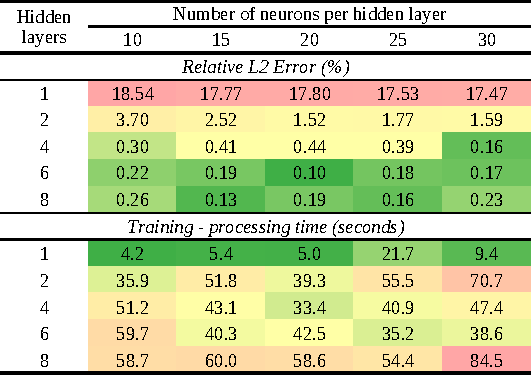
\includegraphics[width=.7\columnwidth]{rlay}
\vspace{1em}
\caption{Relative L2 errors and DNN training times for different number of neurons and hidden layers. On the color scale, the best values are highlighted in green. The simulation ran on the SDumont.}
\label{tab:resu1}
\end{table}

\begin{figure}[htb]\centering
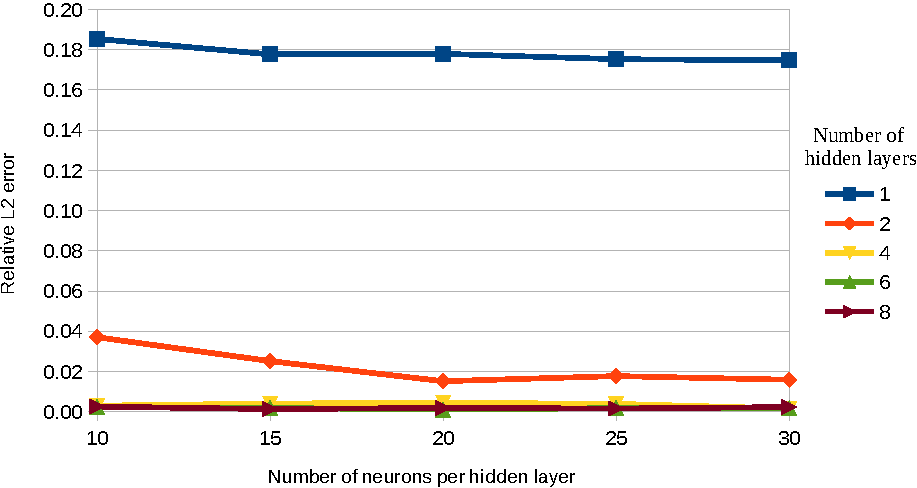
\includegraphics[width=.8\columnwidth]{rlaygrapherror2}
\vspace{0em}
\caption{Relative L2 error (\%) in function of number of neurons and hidden layers. The simulation ran on the SDumont.}
\label{fig:rlaygrapherror2}
\end{figure}

\begin{figure}[htb]\centering
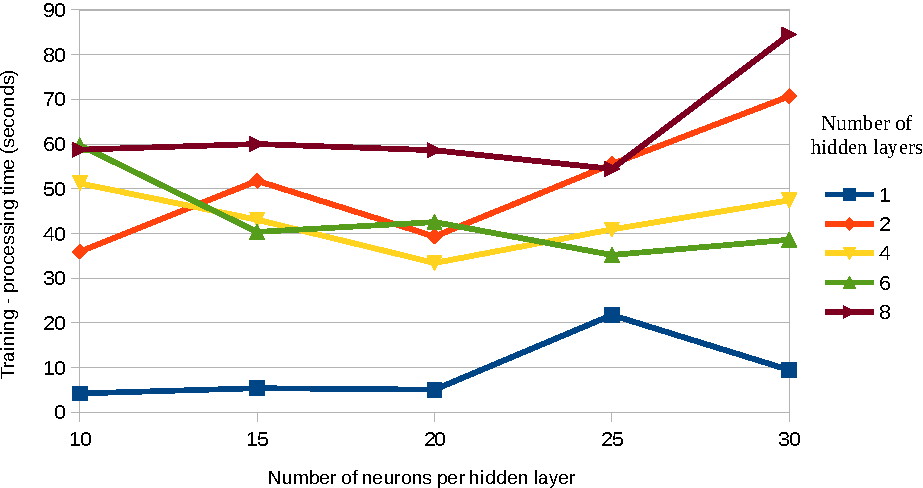
\includegraphics[width=.8\columnwidth]{rlaygraphtime2}
\vspace{0em}
\caption{Processing times (seconds) in function of number of neurons and hidden layers. The simulation ran on the SDumont.}
\label{fig:rlaygraptime2}
\end{figure}

%========================================
\subsubsection{Influence of Neurons and the CP in the PINN}
%========================================

The \autoref{tab:rnu8} shows the relative L2 errors and training times of the PINN, for different hyperparameters and number of CP: 10, 15, 20, 25, and 30 neurons per hidden layer, and 400, 800, 1200, 1600, and 2000 CP. The number of layers was set at 8. All values shown here are the average of 3 runs. In this table, as in the previous one, it is possible to observe that there is a tendency for the best values to be concentrated in the center, probably because the problem of underfitting or overfitting is occurring in the values at the edges of the table. Once again, for future work, it would be interesting to better evaluate this behavior. One of the highlights is that considering the smallest error and the shortest processing time, the best dataset size is 1600, and the best number of neurons per hidden layer is 20.

The \autoref{fig:rnu8graphtime2} shows for most curves a tendency to describe a curve that resembles a parabolic, probably due to the problem of underfitting and overfitting occurring at the beginning and end of the curve. Once again, for future work, it would be interesting to better evaluate this behavior. The shortest processing time occurs for 15 neurons per hidden layer, and 1600 CPs.

The \autoref{fig:rnu8grapherror2} shows that the error for 400 CPs is high compared to the others. 800 CPs presents a significant improvement in accuracy, and the other curves are relatively close, not presenting such a relative large accuracy gain.

\begin{table}[htb]\centering
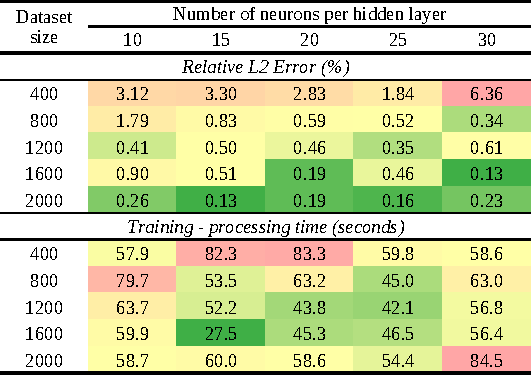
\includegraphics[width=.7\columnwidth]{rnu8}
\vspace{1em}
\caption{Relative L2 errors and DNN training times for different number of neurons and dataset size. The number of hidden layers is set to 8. On the color scale, the best values are highlighted in green. The simulation ran on the SDumont.}
\label{tab:rnu8}
\end{table}

\begin{figure}[htb]\centering
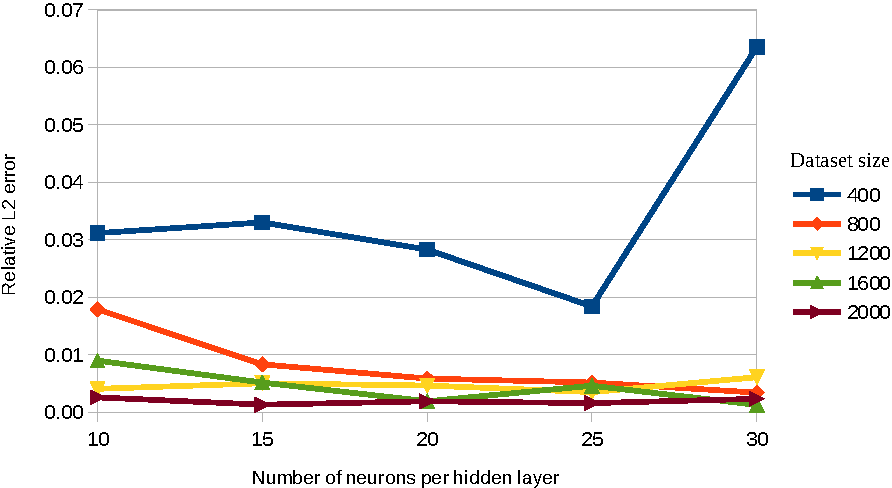
\includegraphics[width=.8\columnwidth]{rnu8grapherror2.pdf}
\vspace{0em}
\caption{Relative L2 error (\%) in function of number of neurons and dataset size. The number of hidden layers is set to 8. The simulation ran on the SDumont.}
\label{fig:rnu8grapherror2}
\end{figure}

\begin{figure}[htb]\centering
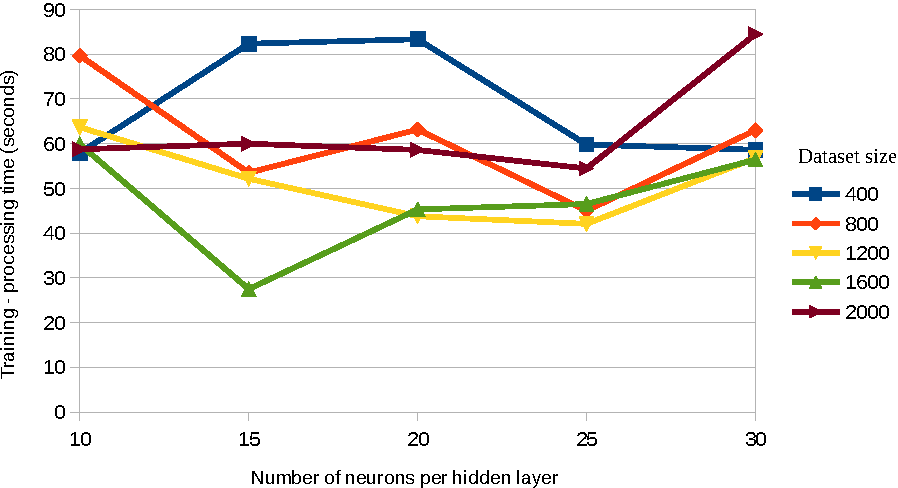
\includegraphics[width=\columnwidth]{rnu8graphtime2.pdf}
\vspace{-1em}
\caption{Processing times (seconds) in function of number of neurons and dataset size. The number of hidden layers is set to 8. The simulation ran on the SDumont.}
\label{fig:rnu8graphtime2}
\end{figure}

%========================================
\subsubsection{PINN Prediction Times}
%========================================

\autoref{tab:rpre} shows the prediction times of the trained PINN model in function of different number of hidden layers (1, 4, 8) and different numbers of neurons per hidden layer (10, 20, 30). As expected, such times are very close, differently from the corresponding training times, which are higher and differ too much. For instance,  in the case of 4 hidden layers and 20 neurons per layer, training time was 33.4 s, while prediction time was only 0.724 s, or 2.2\%. This is a common issue with neural networks, showing the convenience of avoiding re-training the network whenever possible.

\begin{table}[htb]\centering
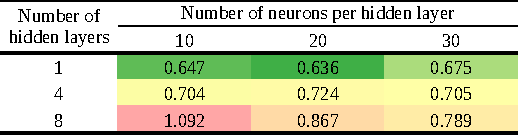
\includegraphics[width=.7\columnwidth]{rpre}
\vspace{1em}
\caption{Prediction times for different number of neurons and hidden layers. On the color scale, the best values are highlighted in green. The simulation ran on the SDumont.}
\label{tab:rpre}
\end{table}






%========================================
%========================================
%========================================
%========================================






\FloatBarrier

%========================================
\section{DNN-Based Gas-Optics Implementation}
\label{sec:resu32}
%========================================

The gas-optical system of the radiation module was implemented using DNN, and the results were compared to those of the implementation using the traditional numerical model. TensorFlow was used to train the DNN, using a dataset derived from various sources. Gprof was used to evaluate the performance of the ecRad versions.


%========================================
%\subsection{DNN-based gas optics model}
%\label{sec:rgom}
%========================================

The result of eCrad running offline with example data is shown in Tables \ref{tab:ecgpr1a} and \ref{tab:ecgpr2a}.
The first table shows the performance analysis of the offline ecRad example with the original numerical scheme, using the gprof tool.
The second table shows the gas-optical DNN version analysis. 
Times are for one run.
The total execution time for the numerical version was 1.55 s, and the time for the DNN version was 1.50 s, showing a performance gain.

\begin{table}[htb]\centering\begin{tabular}{ c c c c c c c } 
\hline
\%	    & cumulative &   self	   &	    &   self	&   total	& \\
time	&  seconds	&  seconds	   & calls	&  ms/call	&  ms/call	& routine \\
\hline
17.42	&      0.27	&     0.27	   & 12	    &    22.50	&    34.06	&  CloudsSW \\
12.90	&      0.47	&     0.20	   & 12	    &    16.67	&    49.17	&  GasOptics \\
12.90	&      0.67	&     0.20	   & 12	    &    16.67	&    30.10	&  CloudsLW \\
9.68	&      0.82	&     0.15	   & 11	    &    13.64	&    13.64	&  Aerosol \\
7.74	&      0.94	&     0.12	   & 4817	&     0.02	&     0.02	&  TransSW \\
\hline \\
\end{tabular}
\caption{The performance analysis using the gprof tool of the offline ecRad example with the original numerical gas-optical scheme. The "routine" column is described in the \autoref{tab:ecgpr1b}. The remaining columns are the standard output of gprof. The total execution time is 1.55 s. Times are for one run.}
\label{tab:ecgpr1a}
\end{table}

\begin{table}[htb]\centering\begin{tabular}{ c c c c c c c } 
\hline
\%	      & cumulative	&   self	&	        &   self	&   total	& \\
time	  &  seconds	&  seconds	&   calls	&  ms/call	&  ms/call	&  routine \\
\hline
16.67	  & 0.25	& 0.25	& 12	& 20.83	& 50.83	& GasOptics \\
16.67	  & 0.50	& 0.25	& 12	& 20.83	& 40.00	& CloudsSW  \\
14.00	  & 0.71	& 0.21	& 832	& 0.25	& 0.25	& TransSW \\
9.33	  & 0.85	& 0.14	& 12	& 11.67	& 11.67	& Aerosol \\
6.00	  & 0.94	& 0.09	& 12	& 7.50	& 20.00	& CloudsLW	\\
\hline \\
\end{tabular}
\caption{The performance analysis using the gprof tool of the offline ecRad example with the DNN gas-optical scheme. The "routine" column is described in the \autoref{tab:ecgpr1b}. The remaining columns are the standard output of gprof. The total execution time is 1.50 s. Times are for one run.}
\label{tab:ecgpr2a}
\end{table}

\begin{table}[htb]\centering\begin{tabular}{ l l }
\hline
routine	    &  name \\
\hline
CloudsSW 	&  \_\_radiation\_tripleclouds\_sw\_MOD\_solver\_tripleclouds\_sw \\
GasOptics	&  \_\_radiation\_ifs\_rrtm\_MOD\_gas\_optics \\
CloudsLW	&  \_\_radiation\_tripleclouds\_lw\_MOD\_solver\_tripleclouds\_lw \\
Aerosol	    &  \_\_radiation\_aerosol\_optics\_MOD\_add\_aerosol\_optics \\
TransSW	    &  \_\_radiation\_two\_stream\_MOD\_calc\_ref\_trans\_sw \\
\hline \\
\end{tabular}
\caption{Complement of the Tables \ref{tab:ecgpr1a} and \ref{tab:ecgpr2a} showing the names of the source files and the names of the routines (gprof standard).}
\label{tab:ecgpr1b}
\end{table}

The "radiation\_ifs\_rrtm" is the interface to IFS implementation of RRTM-G and "gas\_optics" is the gas absorption model implementation. "radiation\_tripleclouds" is the implementation of the "Tripleclouds" SW and LW solver. "radiation\_aerosol\_optics" is the implementation of the aerosol optical properties of the RRTM model. "radiation\_two\_fluxes" is the implementation of the two-flux approximation that simplifies radiative transfer calculations by considering only two primary radiation fluxes, upward and downward irradiance. Comparing the numerical implementation with that using DNN, a point that stands out is the performance increase of the "CloudsLW" LW (thermal-infrared) radiation solver Tripleclouds, which focuses on shallow cumulus clouds and aims to accurately represent the horizontal heterogeneity of subgrid clouds.

In terms of accuracy, the work of \citeonline{Ukkonen2023} shows in the results that the DNN-based model is safe and suitable for use in operational climate and meteorological models. Independent validation of DNN gas optics models was performed using data and methods from CKDMIP \cite{Hogan2020}, using a distinct dataset that was not used in training. The DNN has close accuracy to the scaled-down RRTMGP numerical method used for training, notably in terms of warming rates, and that in both cases it is possible to observe improved bias and RMSE in upward fluxes when employing the DNN. The results for the three CKDMIP concentration scenarios (glacial maximum, pre-industrial and future) are comparable, with the DNN gas optics producing higher upward fluxes and similar warming rates. These preliminary results show a promising path for PIML research.


